\documentclass[a4paper,10pt]{article}

%\usepackage{natbib}
\usepackage{amsthm}
\usepackage{amsfonts}
\usepackage{amssymb}
\usepackage{amsmath}
\usepackage{latexsym}
\usepackage{graphicx}
\usepackage{blindtext}
\usepackage[vietnamese,main=english]{babel}
\usepackage{doc}

\newtheorem*{theorem}{Theorem}
\theoremstyle{definition}
\newtheorem*{definition}{Definition}

\hoffset -1in \topmargin 0mm \voffset 0mm \headheight 0mm
\headsep0mm
\oddsidemargin  20mm     %   Left margin on odd-numbered pages.
\evensidemargin 20mm     %   Left margin on even-numbered pages.
\textwidth   170mm       %   Width of text line.
\textheight  252mm

\makeatletter
\renewcommand\@openbib@code{%
	\advance\leftmargin  \z@ %\bibindent
	\itemindent \z@
	% Move bibitems close together
	\parsep -0.8ex
}
\makeatother

\makeatletter
\renewcommand\section{\@startsection {section}{1}{\z@}%
	{-3.5ex \@plus -1ex \@minus -.2ex}%
	{1.5ex \@plus.2ex}%
	{\large\bfseries}}
\makeatother

\makeatletter
\renewcommand\subsection{\@startsection {subsection}{1}{\z@}%
	{-3.5ex \@plus -1ex \@minus -.2ex}%
	{1.5ex \@plus.2ex}%
	{\normalsize\bfseries}}
\makeatother

\makeatletter
\setlength{\abovecaptionskip}{3pt}   % 0.25cm 
\setlength{\belowcaptionskip}{3pt}   % 0.25cm 
\makeatother

\begin{document}
	\pagestyle{empty}
	
	\begin{center}
		{\bf \Large Automated Optical Inspection in Industry 4.0}
	\end{center}
	
	\smallskip
	\begin{center}
		{\large Hùng Anh Hà Trịnh}
	\end{center}
	
	\smallskip
	\begin{center}
		Faculty of Mechanical Engineering, Brno University of Technology\\
		Institute of Automation and Computer Science\\
		Technicka 2896/2, Brno 616 69, Czech Republic\\
		xhahun00@vutbr.cz\\
	\end{center}
	
	\bigskip
	\noindent Abstract: \textit{This seminary paper deals with the automated optical inspection (AOI) in context of Industry 4.0. First, the term Industry 4.0 and Computer Vision is briefly described and explained. Next, AOI is introduced and hardware and software solutions are presented. In the end, evaluation and conclusion is provided.}
	
	\vspace*{10pt} \noindent Keywords: \textit{industry 4.0, machine learning, deep learning, computer vision, machine vision, automated optical inspection, defect inspection, fault inspection, pcb}
	
	\bigskip
	\section{Introduction}
	\label{sec:1}
	
	In recent years, Industry 4.0 become synonym for modern manufacturing and its future. Manufacturing processes are being modernized and the efficiency is skyrocketing. With increasing demand for electrical devices the need for PCBs is also noticeably growing, thus industry had to adapted. The main question is how?
	
	\section{Industry 4.0}
	\label{sec:2}
	In\,2011, the term \textit{``Industrie\,4.0''} was first introduced during the Hannover Fair. Two years later, the Industry\,4.0 concept was officially presented. The number\,4.0 stands for Fourth Industrial Revolution. \cite{industry_4_0}
	
	Industry 4.0 aims for massive automation and involves technologies and technological developments such as cyber-physical systems, internet of things, robotics, big data, cloud manufacturing and augmented reality. All these technologies together lead to increased efficiency and productivity in manufacturing. \cite{industry_4_0_concepts}
	
	This new paradigm largely impacts production systems, as well as management, economics and society. Even though there are still occurring many challenges and issues, Industry\,4.0 is undoubtedly being integrated by more and more companies not only into manufacturing processes. \cite{industry_4_0}\cite{industry_4_0_concepts}
	
	\begin{figure}[h]
		\begin{center}
			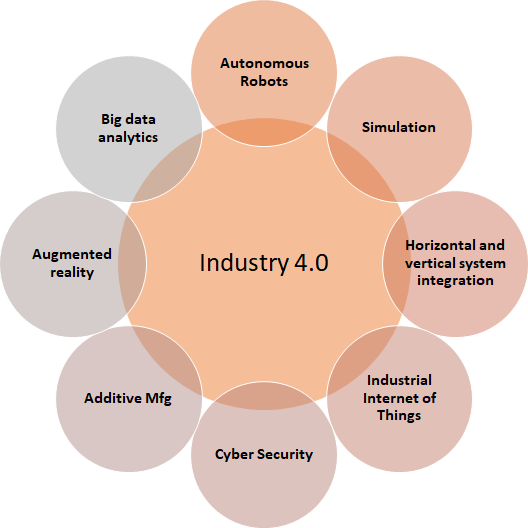
\includegraphics[scale=0.6]{image/i4.png}
			\caption{Technology used in Industry 4.0 (pilot)\cite{industry_4_0_slide}}
			\label{fig:1}
		\end{center}
	\end{figure}
	
	\section{Computer Vision}
	\label{sec:3}
	Computer vision is a interdisciplinary discipline with strong connection to mathematics and computer science as well as to physics. The aim of this field is to provide vision to a computer and make it understand its surroundings, which proves to be a challenging task. One of the main obstacles is the fact, that in computer vision insufficient information is given, thus some unknowns must be recovered to fully specify the solution.
	
	The image is captured as 2D projection of a real 3D object. The transformation to the lower dimension is not lossless, therefore the further the object is to camera, the smaller the object seems in the 2D projection. This way the information about depth was effectively lost.
	
	Unfortunately, noise is present in each measurement in the real world. Images are no exceptions and moreover, as the noise in images is not deterministic, it is much more difficult to effectively get rid of it.
	
	Another problem is the interpretation of the image. Human is able to \textit{``understand''} the image without never ever seeing it before based on previous knowledge and experience. A machine just cannot do this, yet. However, researchers are getting incrementally closer and closer.
	
	As if it was not enough, while working with images, there is one more significant problem and that is the size. Images and especially videos are huge in size, unlike for example text. Although commercially available storage for digital data is getting bigger and processors are getting faster, it is still relevant problem mainly in real-time applications.
	
	Despite all inconveniences, computer vision reached many successes, both in practical and theoretical fields. It is being used in many real-world applications such as optical character recognition, machine inspection, warehouse logistics, medical imaging, biometrics, face detection, self-driving vehicles and many more. \cite{hartley_zisserman}\cite{szeliski}\cite{sonka}
	
	\begin{figure}[h]
		\begin{center}
			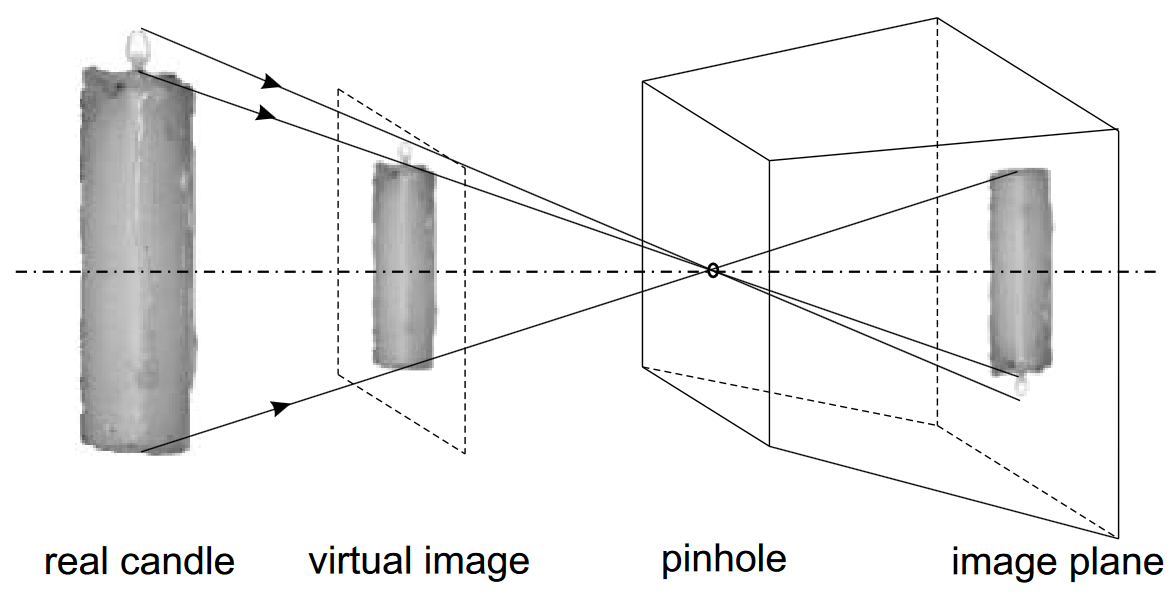
\includegraphics[scale=0.5]{image/cv.png}
			\caption{The pinhole model of imaging geometry\cite{sonka}}
			\label{fig:2}
		\end{center}
	\end{figure}
	
	\section{Components of Automated Optical Inspection}
	\label{sec:4}
	
	Optical inspection is crucial part of printed circuit board manufacturing, since faulty pieces must be effectively identified. It can be done either by a human expert or an automated system. In most cases automated systems have replaced the human experts. With growing popularity of Industry\,4.0, even larger increase in automation can be expected. The automation brings many advantages. Automated optical inspection (AOI) systems relieve human of the endless and exhausting job, so one can concentrate on more human-critical tasks, it is fast and cost efficient, it is also more accurate than human and unlike human, it does not get tired. \cite{richter_streitferdt}\cite{moganti_ercal}
	
	Since AOI system is complex, it consists of many parts. Before applying any inspection algorithm, some hardware requirements must be met.
	
	First, computer, microcomputer or microcontroller on which the algorithm takes place must be defined. All the image classification tasks are carried on the device, thus it has to deal with intense workloads. It is usually a master PC controlling remaining parts. 
	
	Second, image acquisition device with lightning system must be set. It is one of the most important part of the AOI system, if not the most. The quality of acquired images has huge impact on the accuracy of the whole AOI system. It is usually equipped with a variety of illumination modules like user controlled color, ultraviolet or infrared illuminations. \cite{richter_streitferdt}\cite{lu_shi}
	
	It is recommended to set up quality illumination, rather than to make an effort improve computer vision algorithm robustness. A dedicated lightning can facilitate revealing defects and depress the unwanted information. The factors most affecting the imaging quality includes lightning illumination uniformity, luminance or illumination angle. \cite{lu_shi}
	
	\section{Methods of Automated Optical Inspection}
	\label{sec:5}
	
	AOI methods can be basically divided to referential, non-referential and hybrid methods. \cite{moganti_ercal}
	
	\begin{figure}[h]
		\begin{center}
			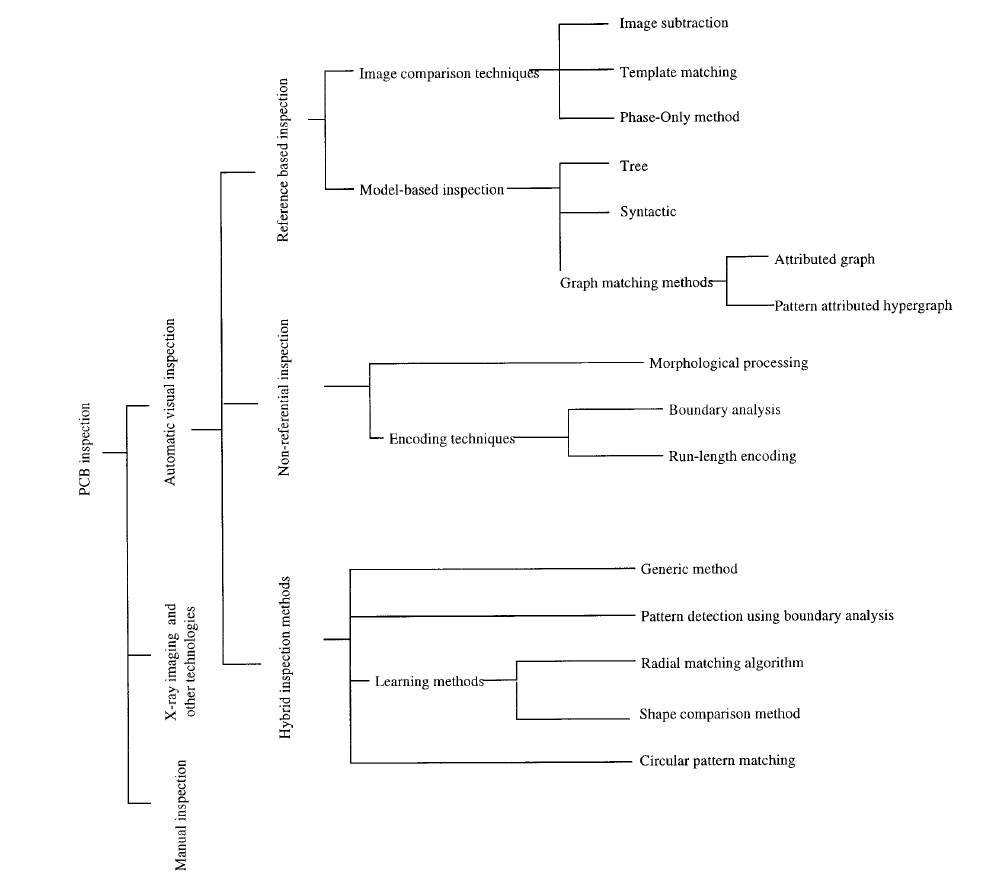
\includegraphics[scale=0.7]{image/aoi.png}
			\caption{Classification of PCB inspection. \cite{moganti_ercal}}
			\label{fig:3}
		\end{center}
	\end{figure}

	\subsection{Referential methods}
	\label{subsec:1}
	As the name of the method may hint, the referential methods are based on point or feature comparison between reference image, also called \textit{``golden image''}, and input image. These methods are able to detect missing tracks, missing termination, opens and shorts. These methods are based on basic image processing operations (like subtraction, XOR, thresholding, and so on), mathematical morphology, two-dimensional HAAR wavelet transform and synthetically generated PCB images. \cite{moganti_ercal}\cite{taha_emary}
	
	\subsection{Non-referential methods}
	\label{subsec:2}
	
	Unlike referential methods, non-referential methods need no reference image nor any pattern. They use design-specification knowledge to inspect the PCB. It inspects specified features like minimum and maximum trace width, circular pad diameters, hole diameters, etc. \cite{moganti_ercal}\cite{taha_emary}
	
	\subsection{Hybrid methods}
	\label{subsec:3}
	
	These methods combine both referential methods and non-referential. Nowadays, these methods are the most effective, however significantly more complex than those previous ones. These methods also include machine learning algorithms.\cite{taha_emary}
	
	In the past few years, computer vision and artificial neural networks made huge progress. With rapidly increasing computational power, the implementation of deep convolutional network in AOI is becoming more common and it brings very convincing results, hence leaving former attempts way behind.
	
	The main difference between deep convolutional network and other machine learning methods lies in engineers not having to extract the features from the image themselves. Since human is error-prone, image features defined by engineers might lack important information needed by the classifier for optimal performance. This problem is solved by deep convolutional network learning the features itself, however huge data sets are needed to effectively train deep neural networks. ANN need high quality training data to achieve great results. \cite{richter_streitferdt}
	
	Lately, several frameworks have been published and used. Few papers comparing the frameworks were written and it is obvious, that each framework suits different application. Some even combined several frameworks, each to perform different task on the same image. \cite{richter_streitferdt}\cite{li_kuo}
	
	\section{Conclusion}
	\label{sec:6}
	Industry 4.0 is still in its beginnings, therefore many new innovations and technologies can be expected to be introduced and even though AOI has been used in industry for decades, it still has not reached its peak. The technology is being improved with enormous speed and right now, improving the deep learning seems to be the next step. 
	
	% References
	%
	\begingroup
	\makeatletter
	\renewcommand\section{\@startsection {section}{1}{\z@}%
		{-3.5ex \@plus -1ex \@minus -.2ex}%
		{4.5ex \@plus.2ex}%
		{\large\bfseries}}
	\makeatother
	
	
	\bibliography{references}{}
	\bibliographystyle{acm}
	\endgroup
	
\end{document}
